% Horizontal (left‑to‑right) flowchart
% Start on the left, decisions/processes flow to the right
\documentclass[tikz,border=2mm]{standalone}
\usetikzlibrary{shapes.geometric, arrows.meta}

\begin{document}

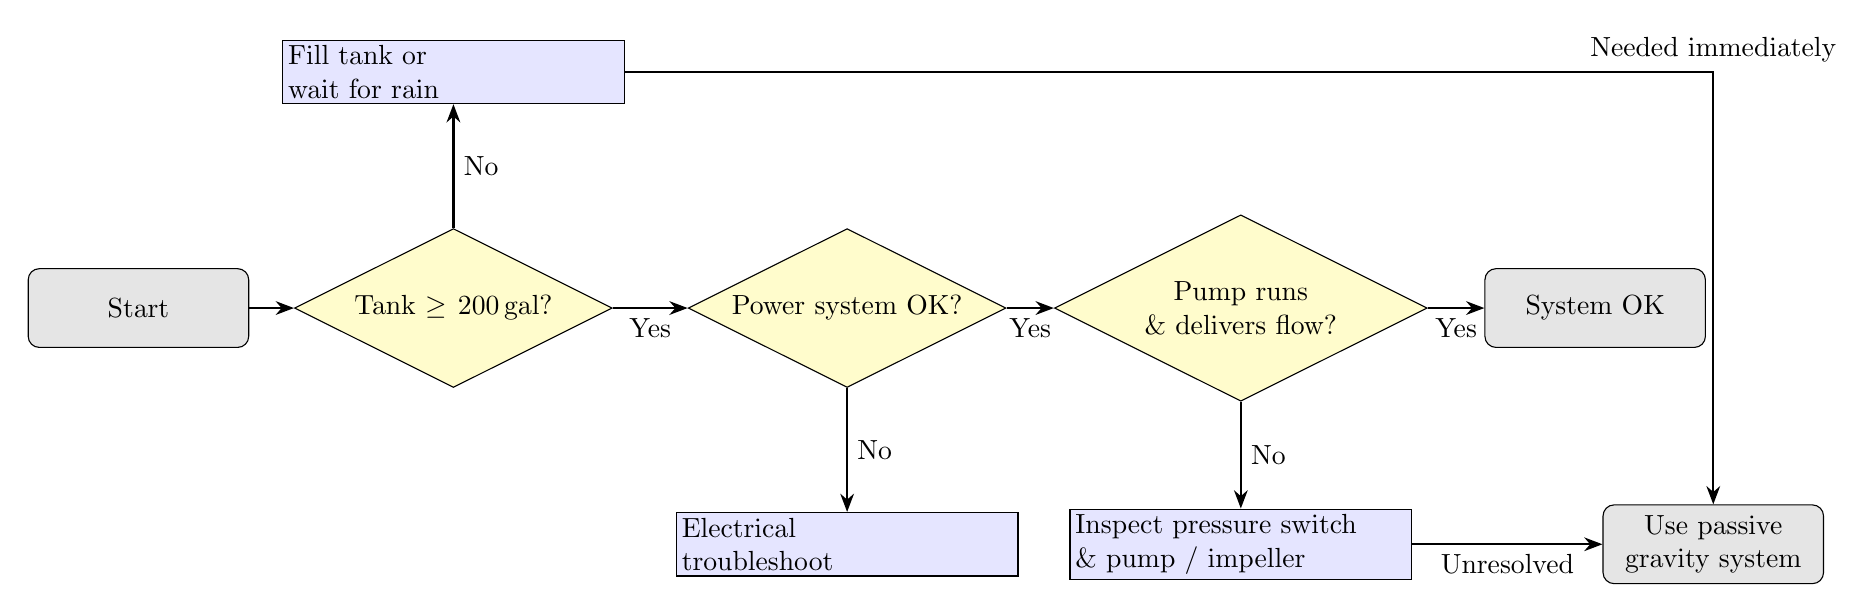
\begin{tikzpicture}[
    >=Stealth,
    startstop/.style = {
        rectangle, rounded corners,
        minimum width = 2.8cm, minimum height = 1cm,
        draw, fill = gray!20, align = center
    },
    decision/.style = {
        diamond, aspect = 2,
        text width = 3.2cm, align = center,
        draw, fill = yellow!20, inner sep = 1pt
    },
    process/.style = {
        rectangle, text width = 4.2cm, align = left,
        draw, fill = blue!10, inner sep = 2pt
    },
    arrow/.style = {thick, ->}
]

% --- Nodes placed by absolute coordinates (cm) ---
\node[startstop] (start)   at ( 0,  0)  {Start};

\node[decision] (tank)     at ( 4,  0)  {Tank $\ge{}200$\,gal?};

\node[process]  (fill)     at ( 4,  3)  {Fill tank or\\wait for rain};

\node[decision] (power)    at ( 9,  0)  {Power system OK?};

\node[process]  (elec)     at ( 9, -3)  {Electrical\\troubleshoot};

\node[decision] (pump)     at (14,  0)  {Pump runs \\ \& delivers flow?};

\node[process]  (inspect)  at (14, -3)  {Inspect pressure switch\\\& pump / impeller};

\node[startstop] (success) at (18.5,  0)  {System OK};

\node[startstop] (passive) at (20, -3)  {Use passive\\gravity system};

% --- Arrows and labels ---
\draw[arrow] (start) -- (tank);

\draw[arrow] (tank)  -- node[below]{Yes} (power);
\draw[arrow] (tank)  -- node[right]{No}  (fill);

\draw[arrow] (fill.east) -| node[above]{Needed immediately} (passive);

\draw[arrow] (power) -- node[below]{Yes} (pump);
\draw[arrow] (power) -- node[right]{No}  (elec);

\draw[arrow] (pump)  -- node[below]{Yes} (success);
\draw[arrow] (pump)  -- node[right]{No}  (inspect);

\draw[arrow] (inspect) -- node[below]{Unresolved} (passive);

\end{tikzpicture}

\end{document}